\documentclass{ximera}
\input{../../preamble}

\addPrintStyle{../..}

\begin{document}
	\author{Bart Lambregs}
	\xmtitle{Bewerkingen met vectoren}{}
    \xmsource\xmuitleg


% SCALAIRE VERMENIGVULDIGING 

% ph: maar met 1 shift vector doen; is veel simpelen -1*(Shift) is de andere
%  TIKZPICTURE DIE DE SCALAIRE VERMENIGVULDIGING ILLUSTREERT 

\subsection*{Scalaire vermenigvuldiging van een reëel getal met een vector}

Wanneer een reëel getal met een vector vermenigvuldigd wordt, dan is er een herschaling van de vector met behoud van richting. 
De grootte en zin kunnen veranderen. Het is een soort reëel veelvoud van de vector. 
De scalarie verminigvuldiging wordt genoteerd als \(\vec{c} = k \cdot \vec{a}\) waarbij \(k \in \R\).

\begin{image}[0.2\textwidth]
\begin{tikzpicture}
    % \draw (-4,-4) grid (4,4);

    \pgfmathsetmacro{\ax}{2}  
    \pgfmathsetmacro{\ay}{0.5}  

    % \pgfmathsetmacro{\c}{$\sqrt{2}$}  
    \pgfmathsetmacro{\d}{2} 

    \coordinate (O) at (0,0); 
    \coordinate (A) at (\ax,\ay); 
    
    \coordinate (Shift) at (0,0.1); 

    \fill (O) circle (2pt); %node[below left]{O};

    \draw[->, very thick,  -latex] (O) -- ($(A)$) node[midway, below]{\(\vec{a}\)};
    \draw[->, very thick,  -latex, blue] ($ (O) - (Shift)$) -- ($-1*(A) - (Shift)$) node[midway, above]{\(-\vec{a}\)};

    \draw[->, very thick,  -latex] ($ (O) + (Shift)$) -- ($\d*(A) + (Shift)$) node[midway, above]{\(2 \cdot \vec{a}\)};
    \draw[->, very thick,  -latex, blue] ($ (O) - 2*(Shift)$) -- ($-0.5*(A) - 2*(Shift)$) node[midway, below]{\(-\frac{1}{2}\vec{a}\)};

\end{tikzpicture}
\end{image}


\subsection*{Samenstelling of som van twee (of meer) vectoren}

Wanneer vectoren van dezelfde grootheid worden opgeteld, bekomt men een nieuwe vector die het netto resultaat is van de samenstelling van de gegeven vectoren. 
Men noemt dit resultaat daarom ook de resultante. Grafisch (kwalitatief) bekomt men de resultante via de kopstaartmethode of parallellogrammethode. 

\begin{image}[0.2\textwidth]
    \begin{tikzpicture}
     % TIKZPICTURE DIE DE SOM VAN TWEE VECTOREN BEREKENT 
    % \draw (-4,-4) grid (4,4);

    \pgfmathsetmacro{\ax}{1}  
    \pgfmathsetmacro{\ay}{2}  
    \pgfmathsetmacro{\bx}{3}  
    \pgfmathsetmacro{\by}{1} 

    \coordinate (O) at (0,0); 
    \coordinate (A) at (\ax,\ay); 
    \coordinate (B) at (\bx,\by); 

    \fill (O) circle (2pt) node[below left]{O};
    % \fill (A) circle (2pt);
    % \fill (B) circle (2pt);

    \draw[->, -latex] (O) -- (A) node[midway, below]{\(\vec{a}\)};
    \draw[->, -latex] (O) -- (B) node[midway, below]{\(\vec{b}\)};
    
    \draw[->, -latex, red, thick] (O) -- ($ (A) + (B)$) node[midway, below]{\(\vec{a} + \vec{b}\)};
    \draw[->, dashed, -latex, red, thick] (A) -- ($ (A) + (B)$) node[midway, below]{\( \vec{b} \)};
    \draw[->, dashed, -latex, red, thick] (B) -- ($ (A) + (B)$) node[midway, below]{\( \vec{a} \)};

\end{tikzpicture}
\end{image}
\captionof{figure}{De optelling van twee vectoren}


De grootte van de resultante bepalen (kwantitatief) kan op verschillende manieren gebeuren, belangrijkste is de meetkundige samenstelling in het oog te houden en zeker niet blindelings de groottes van de gegeven vectoren optellen! 
In evenwijdige of loodrechte gevallen zijn er efficiënte manieren om de resultante te bepalen (som/verschil of stelling van Pythagoras), de meest algemene methode is echter met de (gewijzigde) cosinusregel:

\[
\vec{c} = \vec{a} + \vec{b} \Rightarrow \| \vec{c} \|^2 = \| \vec{c} \|^2 + \| \vec{c} \|^2 + 2 \cdot \|\vec{a}\| \cdot \|\vec{b}\| \cdot \cos(\alpha)
\]

met \(\alpha\) de hoek tussen \(\vec{a}\) en \(\vec{b}\). 

\begin{example}

In onderstaande figuur is \(\|\vec{a}\| = \SI{3}{\newton}\) en \(\|\vec{b}\| = \SI{5}{\newton}\). 
Bijgevolg is  \(\| \vec{c} \| = \|\vec{a}\| + \|\vec{b}\| = \SI{8}{\newton}\). 

\begin{image}[0.2\textwidth]
    \begin{tikzpicture}
        \coordinate (O) at (0,0);
        \coordinate (A) at (1,0);
        \coordinate (B) at (2,0);
        \coordinate (C) at (3,0);

        \coordinate (Shift) at (0,0.05);

        \fill (O) circle (1pt);
        \fill ($ (O) + (Shift) $) circle (1pt);
        \fill ($ (O) - (Shift) $) circle (1pt);


        \draw[->] ($ (O) + (Shift) $)--($ (A) + (Shift) $)  node[midway, above]{$\vec{a}$};
        \draw[->] (O)--(C)                                  node[pos=0.7, above]{$ \vec{c} = \vec{a} + \vec{b} $};
        \draw[->] ($ (O) - (Shift) $)--($ (B) - (Shift) $)  node[midway, below]{$\vec{b}$};
    \end{tikzpicture}
\end{image}
\end{example}

\begin{example}

% hier staat onnauwkeurigheid; de norm moet buiten de bewerking staan; de norm van een verschil is commutatief

In onderstaande figuur is \(\|\vec{a}\| = \SI{3}{\newton}\) en \(\|\vec{b}\| = \SI{5}{\newton}\). 
Bijgevolg is  \(\| \vec{c} \| = \|\vec{a} + \vec{b}\| = \| -3 + 5 \| = \SI{2}{\newton}\). 

\begin{image}[0.2\textwidth]
    \begin{tikzpicture}
        \coordinate (O) at (0,0);
        \coordinate (A) at (-1,0);
        \coordinate (B) at (2,0);
        \coordinate (C) at (1,0);

        \coordinate (Shift) at (0,0.05);

        \fill (O) circle (1pt);
        \fill ($ (O) + (Shift) $) circle (1pt);
        \fill ($ (O) - (Shift) $) circle (1pt);


        \draw[->] ($ (O) + (Shift) $)--($ (A) + (Shift) $)  node[midway, above]{$\vec{a}$};
        \draw[->] (O)--(C)                                  node[pos=0.7, above]{$ \vec{c} = \vec{a} + \vec{b} $};
        \draw[->] ($ (O) - (Shift) $)--($ (B) - (Shift) $)  node[midway, below]{$\vec{b}$};
    \end{tikzpicture}
\end{image}
\end{example}



\begin{example}
    \begin{image}[0.2\textwidth]
        \begin{tikzpicture}
            % TIKZPICTURE DIE DE SOM VAN TWEE VECTOREN BEREKENT 
           % \draw (-4,-4) grid (4,4);
       
           \pgfmathsetmacro{\ax}{1}  
           \pgfmathsetmacro{\ay}{2}  
           \pgfmathsetmacro{\bx}{3}  
           \pgfmathsetmacro{\by}{1} 

           \pgfmathsetmacro{\ang}{50} 
       
           \coordinate (O) at (0,0); 
           \coordinate (A) at (\ang :1); 
           \coordinate (B) at (0:1.5); 
           \coordinate (C) at ($ (A) + (B)$); 
           
           \coordinate (Z) at (180:1); 

           \draw[dotted] (O)--(Z);
       
           \draw[->, -latex, blue] (O) -- (A) node[midway, above left]{\(\vec{a}\)};
           \draw[->, -latex, red] (O) -- (B) node[midway, below]{\(\vec{b}\)};
           \draw[->, -latex, green] (O) -- (C) node[pos=1, above right, green]{\(\vec{c} = \vec{a}+\vec{b}\)};
           
           \draw[->, dashed, -latex, red, thick] (A) -- (C) node[midway, above left]{\( \vec{b} \)};
           \draw[->, dashed, -latex, blue, thick] (B) -- (C) node[midway, below right]{\( \vec{a} \)};
       
       \end{tikzpicture}
    \end{image}
\end{example}






% ONTBINDEN IN COMPONENTEN 


% TIKZPICTURE DIE DE ONTBINDING IN COMPONENTEN WEERGEEFT 
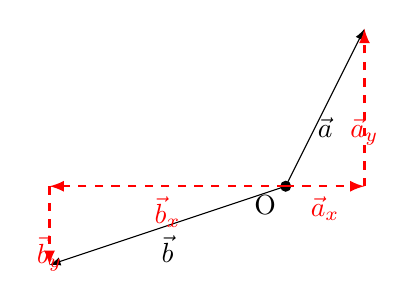
\begin{tikzpicture}
    % \draw (-4,-4) grid (4,4);

    \pgfmathsetmacro{\ax}{1}  
    \pgfmathsetmacro{\ay}{2}  
    \pgfmathsetmacro{\bx}{-3}  
    \pgfmathsetmacro{\by}{-1} 

    \coordinate (O) at (0,0); 
    \coordinate (A) at (\ax,\ay); 
    \coordinate (B) at (\bx,\by); 

    \fill (O) circle (2pt) node[below left]{O};
    % \fill (A) circle (2pt);
    % \fill (B) circle (2pt);


    \draw[->, -latex] (O) -- (A) node[midway, below]{\(\vec{a}\)};
    \draw[->, dashed, -latex, red, thick] (O) -- (\ax, 0) node[midway, below]{\( \vec{a}_x \)};
    \draw[->, dashed, -latex, red, thick] (\ax, 0) -- (A) node[midway, below]{\( \vec{a}_y \)};
    
    
    \draw[->, -latex] (O) -- (B) node[midway, below]{\(\vec{b}\)};
    \draw[->, dashed, -latex, red, thick] (O) -- (\bx, 0) node[midway, below]{\( \vec{b}_x \)};
    \draw[->, dashed, -latex, red, thick] (\bx, 0) -- (B) node[midway, below]{\( \vec{b}_y \)};
    
\end{tikzpicture}


% SCALAIR PRODUCT 

% TIKZPICTURE DIE SCALAIR PRODUCT van a op b ILLUSTREERT  
\begin{tikzpicture}
    % \draw (-4,-4) grid (4,4);

    \pgfmathsetmacro{\ax}{1}  
    \pgfmathsetmacro{\ay}{2}  
    \pgfmathsetmacro{\bx}{3}  
    \pgfmathsetmacro{\by}{0} 

    \coordinate (O) at (0,0); 
    \coordinate (A) at (\ax,\ay); 
    \coordinate (B) at (\bx,\by); 

    \fill (O) circle (2pt) node[below left]{O};
    
    \draw[->, -latex] (O) -- (B) node[midway, below]{\(\vec{b}\)};

    \draw[->, -latex] (O) -- (A) node[midway, above left]{\(\vec{a}\)};
    \draw[->, dashed, -latex, red, thick] (O) -- (\ax, 0) node[midway, below]{\( \vec{a}_x \)};
    \draw[dashed, -latex, thick] (\ax, 0) -- (A);


    \draw pic[ pic text= $\theta$, draw,  angle radius=0.7cm]{angle = B--O--A};
    
        
\end{tikzpicture}


% VECTORIEEL PRODUCT 

\end{document}
